\section{Scaling Time}


\begin{figure}[htpb]
    \centering
    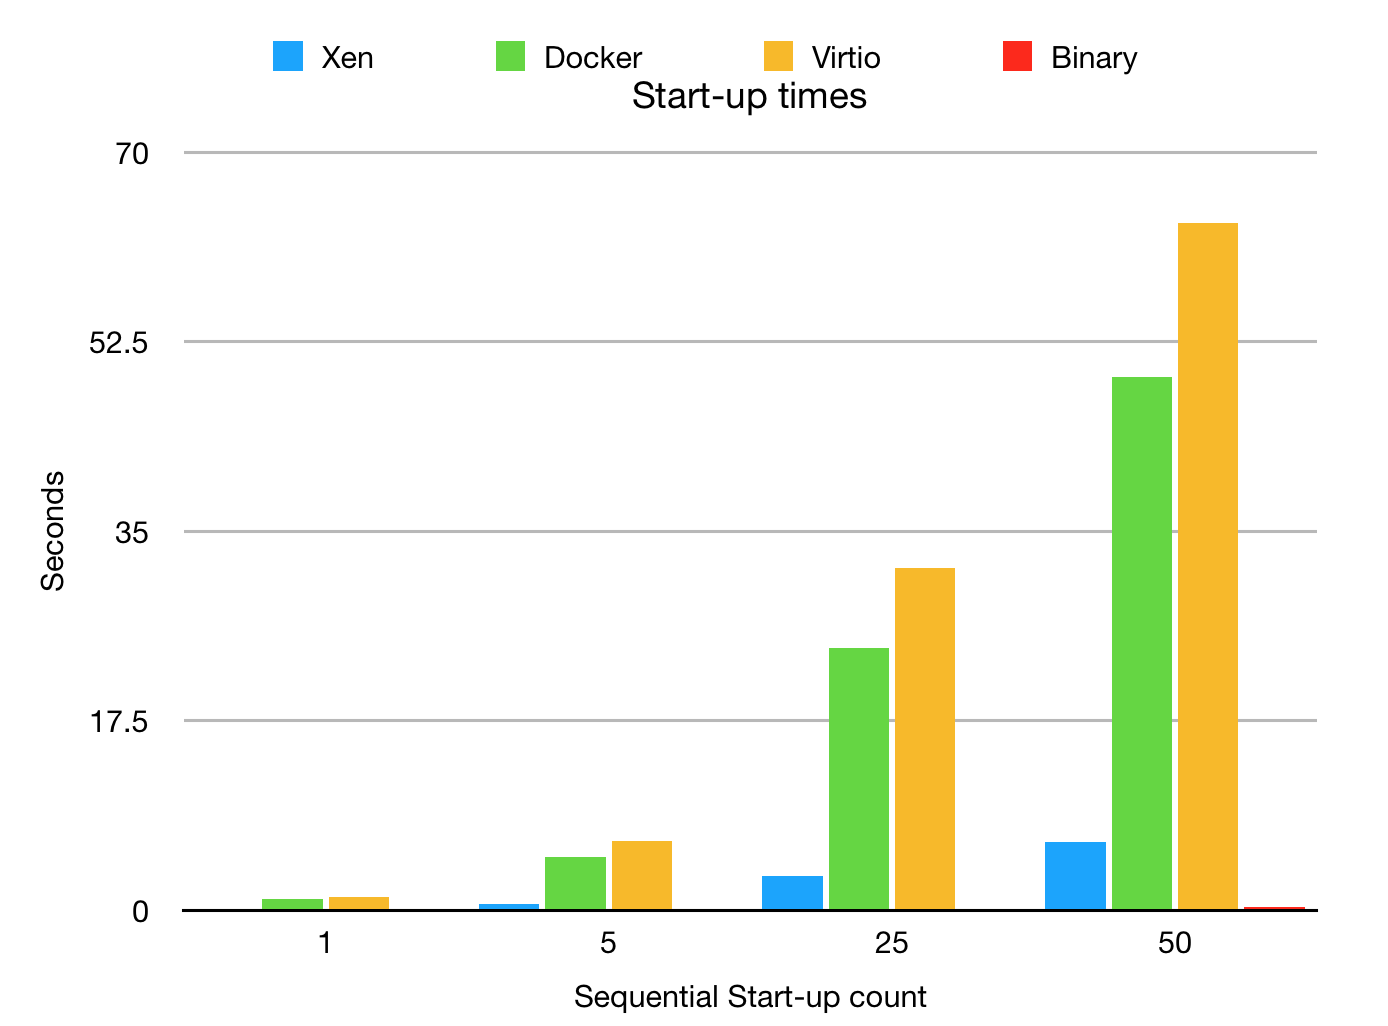
\includegraphics[width=1\textwidth]{figures/boot-speed.png}
    \caption{Boot Speed Comparison } \label{fig:boot}
  \end{figure}
  
  
  \pgfplotstableread[row sep=\\,col sep=&]{
      count & docker & unikernel \\
      1     & 1.146  & 0.015   \\
      4     & 5.384 & 0.066    \\
      25    & 35.081 & 0.335  \\
      50   & 70.987 & 0.646  \\
      }\mydata
\begin {figure}[htpb]
\centering
  \begin{tikzpicture}
      \begin{axis}[
              ybar,
              bar width=.5cm,
              width=\textwidth,
              height=.5\textwidth,
              legend style={at={(0.5,1)},
                  anchor=north,legend columns=-1},
              symbolic x coords={1,4,25,50},
              xtick=data,
              nodes near coords,
              nodes near coords align={vertical},
              ymin=0,ymax=80,
              ylabel={Seconds},
              xlabel={Sequential boot count}
          ]
          \addplot table[x=count,y=docker]{\mydata};
          \addplot table[x=count,y=unikernel]{\mydata};
          \legend{Docker, Unikernel}
          
      \end{axis}
  \end{tikzpicture}
  \caption{Boot Time on Mac os }\label{fig:boot-time}
\end{figure}